\section{Experiments}
\label{sec:exp}
\subsection{Data}
\label{sec:data}
The main data are MTEB result files at the pinned commit (text-embedding models $\times$ embedding tasks; speed tasks and scores outside $[-1,1]$ removed, test split preferred, \texttt{main\_score} averaged over subsets, revisions of a model merged). The raw matrix is $12\%$ observed and its missingness is tied to benchmark version and release date, so we evaluate on blocks that are nearly complete and treat density as an axis: \texttt{mteb-dense56} (tasks scored by $\ge200$ models), \texttt{mteb-dense} (275 tasks), \texttt{mteb-mid} (357) and \texttt{mteb-sparse} (472 tasks, $30\%$ observed). The dense blocks are not a random sample: \texttt{mteb-dense56} keeps $28\%$ of the models and $4\%$ of the tasks of the raw leaderboard ($10\%$ of its observed cells; median release year 2024, median $245$M parameters; Appendix~\ref{app:extra}), so the results concern models that were run on a common core of tasks. HELM-MMLU (57 subjects), HELM Lite extended (91 models $\times$ 28 scenarios, built from the pinned HELM Lite v1.13.0 exports), HELM Lite (10 scenarios), LiveBench (7 categories) and the Open LLM Leaderboard (6 benchmarks) are generative-LLM matrices; each is analysed on its own (no cross-leaderboard name matching). The pinned Open LLM Leaderboard and LiveBench exports give only six and seven benchmarks, so these stay small-$N$ (Appendix~\ref{app:repro}). Nine real matrices are reported (four MTEB, five generative-LLM). Synthetic rank-$r$ matrices with known truth are used for theory and condition checks only.

\subsection{How accurate is inference from $k$ benchmarks, and how do the rules compare?}
\begin{figure}[t]
\centering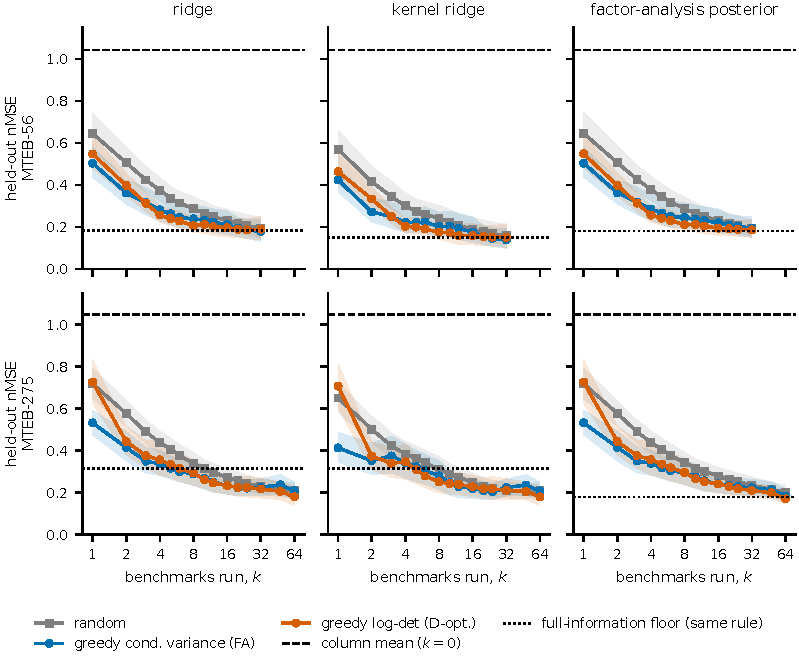
\includegraphics[width=0.55\linewidth]{fig1_main_curves.pdf}
\caption{Held-out nMSE against the number $k$ of benchmarks run (protocol B, random 10-fold CV, 95\% bootstrap bands over held-out models) on MTEB-56 (152 models $\times$ 56 tasks, top) and MTEB-275 (133 $\times$ 275, bottom). Random selection and two greedy selectors fitted on training models, for three inference rules. Dashed: column-mean predictor; dotted: full-information floor of the same rule.}
\label{fig:main}
\end{figure}
Figure~\ref{fig:main} gives the central result. Predicting the training mean gives $\nmse\approx1.04$ (RMSE $15.0$ score points) on MTEB-56. With $k=4$ benchmarks run and kernel-ridge inference, the error falls to $0.30$ for random selection and to $0.22$ (greedy conditional variance) or $0.20$ (greedy log-det), i.e.\ RMSE $7.8$, $6.8$ and $6.6$ points; the full-information floor of the same rule is $0.15$. The curves flatten around $k\approx8$--$16$ and the informed and random curves meet by $k\approx 16$--$32$. On MTEB-275 the picture is the same with a higher floor ($0.18$ for the factor posterior, $0.32$ for kernel ridge, which has more inputs than informative training models in the full-information case). The inference rule matters at least as much as selection (Table~\ref{tab:cross}, Appendix; $k=4$, random selection): the single-aggregate regression (\texttt{avgreg}) has $0.48$ against $0.30$ for kernel ridge, whereas kernel ridge with greedy log-det instead of random gains $0.10$; the single-score baseline stays at $0.40$--$0.41$ even at $k=16$ (its floor is $0.40$), so one ``general ability'' number cannot reproduce the other benchmarks here.

\subsection{Does informed selection beat random selection?}
\begin{figure}[t]
\centering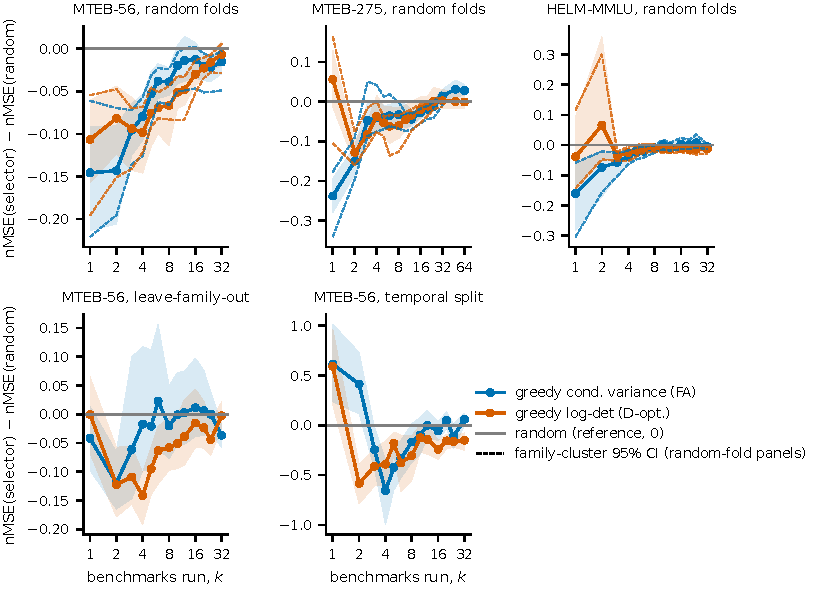
\includegraphics[width=0.55\linewidth]{fig3_paired_vs_random.pdf}
\caption{Paired difference in nMSE between an informed selector and random selection (kernel-ridge inference, same held-out models; below 0 favours the informed selector; paired 95\% bootstrap bands over held-out models; dashed: strict-family bootstrap, random-fold panels). Random folds on three matrices, then leave-family-out and temporal splits (one fold of about 30 newest models) on MTEB-56.}
\label{fig:paired}
\end{figure}
Yes, at small $k$, and not beyond a moderate $k$ (Fig.~\ref{fig:paired}). On MTEB-56 greedy conditional-variance selection improves on random by $0.15$ (95\% CI $0.09$--$0.21$) at $k=1$--$2$, by $0.08$ ($0.05$--$0.11$) at $k=4$ and $0.04$ at $k=8$; at $k=16$ the gain is not distinguishable from zero ($-0.012$, CI $-0.034$ to $0.008$). Log-det selection gives $-0.10$ at $k=4$ and remains significant at $k=16$ ($-0.030$, CI $-0.043$ to $-0.018$) but not at $k=32$. On MTEB-275 the gain at $k=1$ is $0.24$, falls to $0.04$ at $k=4$ (CI includes $0$) and is slightly \emph{negative} ($+0.014$) at $k=32$; on HELM-MMLU it is $0.16$ at $k=1$ and $0.04$ at $k=4$, and on the 91-model HELM Lite matrix $0.18$, $0.11$, $0.12$, $0.05$ at $k=1,2,4,8$. These intervals bootstrap models; resampling organisations or strict families widens the paired intervals by about $10$--$25\%$ at $k\le2$ and keeps the sign of every difference up to $k=8$ on MTEB-56 (families: $k=1$ $-0.146$, CI $-0.221$ to $-0.061$; $k=8$ $-0.039$, $-0.066$ to $-0.024$), whereas from $k=12$ the interval contains $0$. The benefit is largest where the budget is smallest, as the model-based theory predicts.

Not every selection heuristic helps: leverage-score, pivoted-QR and highest-variance selection, the standard column-subset-selection choices, are \emph{worse} than random at $k\le8$ (at $k=4$ with kernel ridge: $0.38$, $0.37$, $0.38$ against $0.30$ for random, Tables~\ref{tab:cross}, \ref{tab:crossall}), as is $k$-center ($0.34$). A diagnostic points to rank mismatch rather than redundancy: at the cross-validated rank their picks are \emph{less} mutually correlated than random ones but have high task-specific variance (noisy tasks), and with the rank fixed at $3$ they reach $\nmse\le0.5$ at $k=3$ instead of $4$--$6$ (Appendix~\ref{app:extra}). Picking the benchmarks most correlated with the others (``most central'') behaves differently: it is as good as the informed selectors at $k=1$--$2$ on MTEB-56 (paired difference to random $-0.13$ and $-0.09$, against $-0.15$, $-0.14$ for conditional variance) and on MTEB-275 ($-0.22$, $-0.12$), is indistinguishable from random at $k=4$ and $k=16$, and on MTEB-275 and HELM-MMLU is \emph{worse} than random at $k=8$--$16$ ($+0.05$; $+0.04$). Direct paired contrasts (kernel ridge, family-clustered bootstrap; Appendix Figs.~\ref{fig:clpaired}, \ref{fig:xbase}, Tables~\ref{tab:xsel}--\ref{tab:xselpaired}) show that it is worse than conditional variance at $k=2$--$4$ on MTEB-56 ($+0.06$; and against random only $k=1$ stays separated from zero for $k\le8$ once families are resampled) and at $k=8$--$16$ on MTEB-275, that conditional variance and log-det are not separated at $k\le4$ and that log-det is better from $k\ge8$ ($+0.03$ for conditional variance minus log-det). Conditional variance is not the best deployable selector either: forward ridge selection of a shared set (\texttt{fwd\_ridge}) and a greedy rule that re-estimates a local Gaussian after each revealed score (\texttt{adapt\_loc}) are better by about $0.03$--$0.04$ at $k=8$--$16$ on MTEB-56,; none is uniformly best, and on HELM-MMLU the informed selectors are within $0.04$ of each other at $k\ge4$.

An oracle that picks benchmarks using the held-out model's own target scores (an optimistic upper bound; Table~\ref{tab:oracle}, Fig.~\ref{fig:oracle}a) reaches $0.29$ and $0.23$ at $k=1,2$ on MTEB-56 against $0.42$/$0.27$ for greedy conditional variance and $0.57$/$0.42$ for random, so a real gap to ideal selection remains at the smallest budgets and is small from $k=4$. Fitting the selection model on the held-out rows as well (peeking) lowers the error of conditional-variance selection at $k=4$ from $0.22$ to $0.19$ (Fig.~\ref{fig:oracle}b); selection is fitted on training models only everywhere else, so the reported gains are free of this optimism.

\subsection{How large must $k$ be?}
\begin{table}[t]
\caption{Smallest $k$ whose 95\% bootstrap lower bound of the gap-closed fraction $G(k)$ reaches $0.8$ and $0.9$ (criterion fixed before the final runs; floor = same inference rule with all non-target benchmarks revealed, value in column ``floor''; ``rand.'', ``GV'' = greedy conditional variance, ``D-opt'' = greedy log-det). krr: kernel ridge, fa: factor-analysis posterior. Grids: $k\in\{1,2,\dots,6,8,10,12,16,20,24,32,48,64\}$ where $N$ allows.}
\label{tab:kstar}
\centering\scriptsize\setlength{\tabcolsep}{2.5pt}
\begin{tabular}{llrrrrrrr}
\toprule
 & & & \multicolumn{3}{c}{$G\geq0.8$} & \multicolumn{3}{c}{$G\geq0.9$} \\
\cmidrule(lr){4-6}\cmidrule(lr){7-9}
dataset & rule & floor & rand. & GV & D-opt & rand. & GV & D-opt \\
\midrule
mteb-dense56 & krr & 0.15 & 5 & 2 & 3 & 12 & 8 & 4 \\
mteb-dense56 & fa & 0.18 & 8 & 4 & 3 & 16 & 16 & 5 \\
mteb-dense & krr & 0.32 & 3 & 1 & 2 & 6 & 5 & 3 \\
mteb-dense & fa & 0.18 & 10 & 6 & 8 & 32 & 16 & 20 \\
mteb-mid & krr & 0.35 & 3 & 2 & 2 & 5 & 3 & 3 \\
mteb-mid & fa & 0.17 & 16 & 8 & 12 & 48 & 24 & 32 \\
mteb-sparse & krr & 0.43 & 3 & 2 & 4 & 5 & 3 & 4 \\
mteb-sparse & fa & 0.18 & 16 & 16 & 24 & 48 & 32 & 24 \\
helm-mmlu & krr & 0.28 & 2 & 1 & 3 & 3 & 1 & 3 \\
helm-mmlu & fa & 0.21 & 3 & 1 & 3 & 5 & 3 & 4 \\
helm & krr & 0.26 & 4 & 2 & 2 & 6 & 3 & 5 \\
helm & fa & 0.36 & 5 & 2 & 2 & 6 & 2 & 2 \\
helm-lite-ext & krr & 0.35 & 5 & 2 & 3 & 8 & 4 & 4 \\
helm-lite-ext & fa & 0.31 & 8 & 3 & 4 & 12 & 5 & 5 \\
livebench & krr & 0.34 & 1 & 1 & 1 & 2 & 2 & 2 \\
livebench & fa & 0.32 & 2 & 2 & 2 & 3 & 3 & 2 \\
olb & krr & 0.29 & 2 & 1 & 1 & 3 & 1 & 1 \\
olb & fa & 0.34 & 2 & 1 & 1 & 3 & 1 & 1 \\
\bottomrule
\end{tabular}

\end{table}
Table~\ref{tab:kstar} reports $k^\star$ under the pre-fixed criterion. On MTEB-56, $k^\star(0.8)$ is $2$ for greedy conditional variance and $3$ for log-det with kernel ridge, against $5$ for random selection; $k^\star(0.9)$ is $8$/$4$ against $12$. With the factor posterior the corresponding numbers are $4$/$3$ against $8$ for $G\ge0.8$ and $16$/$5$ against $16$ for $G\ge0.9$. On the larger MTEB matrices more benchmarks are needed for the better-floored factor posterior ($k^\star(0.8)=6$--$12$ for informed selection, $10$ and $16$ for random; $k^\star(0.9)=16$--$48$), and on the small generative-LLM matrices ($N=6$--$57$) $k^\star(0.8)\le 4$ in all but one row --- limited by $N$. $k^\star$ is relative to what the rule could achieve with everything revealed, and that floor is itself far from zero ($0.15$--$0.43$). With absolute tolerances (Appendix, Table~\ref{tab:kstar-abs}) $\nmse\le0.5$ needs $k\le5$ in all MTEB dense rows and $\nmse\le0.25$ needs $k=4$--$64$. $k^\star$ is a step function of noisy curves, so we report its spread (Appendix Tables~\ref{tab:kstarcl}, \ref{tab:kstarsplit}). Resampling organisations or strict families instead of models leaves $k^\star(0.8)$ unchanged for random ($5$) and log-det ($3$) and raises it for conditional variance ($2\to3$); its point value is $2$ in all three repetitions against $4,4,4$ for random. Under shift the ranking among informed selectors is not stable (kernel ridge, MTEB-56, $G\ge0.8$; conditional variance / log-det / random): random folds $2/3/5$, organisation leave-out $8/3/6$, strict-family leave-out $2/8/6$, temporal $4/2/6$. Under shift conditional variance beats random robustly only at $k\le3$.
The answer to ``how large $k$'' is therefore: a handful of benchmarks ($2$--$4$ for $80\%$ and $4$--$16$ for $90\%$ of the gap on MTEB-56, i.e.\ $4$--$29\%$ of $N$) recovers most of the gain over the mean, but a few tens are needed to approach the accuracy that all other benchmarks would give, and there is no sharp elbow, in line with the intermediate effective rank of these matrices (Table~\ref{tab:data}, Appendix).

\subsection{Data conditions and distribution shift}
\paragraph{Missingness, $M$, rank (Appendix Fig.~\ref{fig:cond}).} Removing $30\%$ or $60\%$ of the training cells raises the error of greedy conditional variance with kernel ridge at $k=4$ from $0.22$ to $0.27$ and $0.38$ (random: $0.34$, $0.48$): selection still helps, but the error degrades. With $M=60$, $30$, $15$ training models the error is $0.26$, $0.46$, $0.93$ ($k=4$); the training set must be several times larger than $k$. Fixing the factor rank at 2, 4 or 8 changes nMSE at $k=16$ by at most $0.02$.\par\paragraph{A sparse leaderboard.} On \texttt{mteb-sparse} ($479\times472$, $30\%$ observed; a new model reveals the first $k$ benchmarks of the ordering that it has scores for, and models with fewer than $k$ scores are skipped for that $k$) the column mean has nMSE $1.06$ and the best full-information rule (factor posterior) $0.18$. Conditional variance with the factor posterior gives $0.59/0.45/0.37/0.30$ at $k=2/4/8/16$ against $0.65/0.52/0.42/0.33$ for random selection; the paired gain is separated from zero up to $k=8$ ($-0.083$ at $k=4$) but not at $k\ge16$, and log-det is worse than random at $k\le4$. $k^\star(G\ge0.8)$ with the factor posterior is $16$ for conditional variance and random selection and $24$ for log-det, so about $16$ benchmarks are needed and informed selection no longer shortens it; kernel ridge reaches the criterion at $k=2$--$4$ only because mean imputation makes its own floor poor ($0.43$; Appendix~\ref{app:extra}).
\paragraph{Different matrices.} All matrices have a dominant first component ($36$--$80\%$ of variance) but participation-ratio ranks of only $1.6$--$3.2$ against hold-out-optimal factor ranks of $3$--$16$ (Appendix Table~\ref{tab:data}); the small HELM-MMLU and Open LLM Leaderboard matrices hit their floors after $k\approx3$--$4$. The gain from selection is clear on the Open LLM Leaderboard ($0.16$ at $k=1$) and HELM Lite ($0.16$--$0.19$ at $k\le2$) but not distinguishable from zero on LiveBench at $k\le2$, and weak on MTEB-357 beyond $k=8$. Selection conclusions thus hold at $k\le4$ across both families, but the generative-LLM curves are short.
\begin{figure}[t]
\centering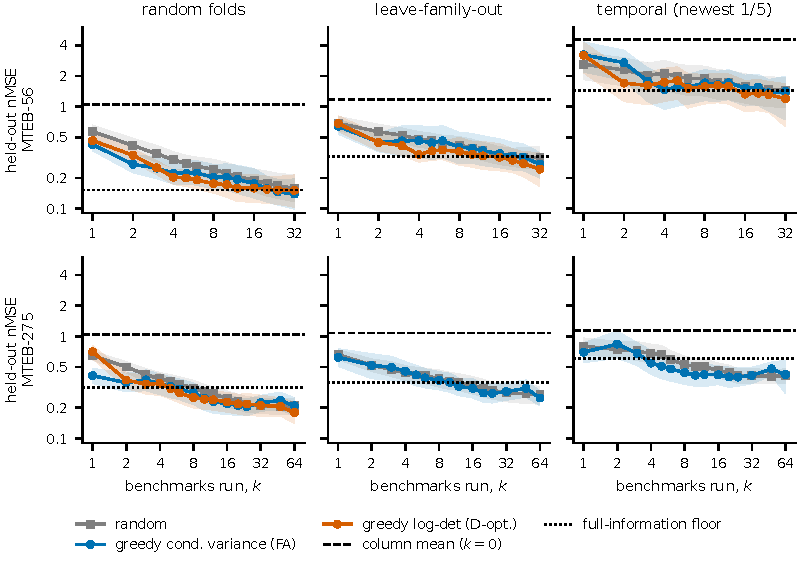
\includegraphics[width=0.55\linewidth]{fig5_shift.pdf}
\caption{Held-out nMSE (kernel ridge, log axis) under random folds, leave-family-out and temporal splits on MTEB-56 (top) and MTEB-275 (bottom). The temporal split has one fold of about 30 test models; its intervals reflect those models only.}
\label{fig:shift}
\end{figure}
\paragraph{Shift (Fig.~\ref{fig:shift}).} When whole families (organisations) are held out, the column-mean error rises to $1.18$ and the full-information floors to $0.27$--$0.33$ (from $0.15$--$0.18$); at $k=16$ kernel ridge reaches $0.33$ (random) against $\approx0.19$ in random folds. Informed selection still helps at $k=2$ (log-det $-0.12$, CI $-0.18$ to $-0.06$), at $k=4$ only for log-det ($-0.14$; conditional variance $-0.02$, CI $-0.10$ to $0.12$), and not for $k\ge16$. The temporal split is the clear failure case: the newest models lie outside the range of older ones, the column mean reaches $4.6$ and even the full-information floor is $1.4$--$1.5$, so no budget of $k\le32$ gives an error below $1.2$ (log-det) on MTEB-56; on MTEB-275 the newest models are better predicted ($0.42$ at $k=16$ against $1.14$ for the mean). Neither remedy we tried changes this: a release-date covariate, or unshrunk least squares instead of the factor posterior, changes nMSE by at most $0.05$ on the single temporal fold (MTEB-56, $k=2/4/8/16$: posterior $1.96/1.50/1.56/1.49$, with trend $1.91/1.46/1.55/1.50$). In a rolling-origin evaluation (four cutoffs) the posterior with conditional-variance selection gives $0.96/0.91/0.87/0.74$ against $2.18$ for the mean, and informed selection beats random at $k=2$ ($1.25$) but not at $k=16$ (Appendix Table~\ref{tab:drift}). A Mahalanobis check on the $k$ revealed scores under the training covariance (flag at the $95\%$ $\chi^2$ level) flags $7$--$8\%$ of models in random folds, $5$--$15\%$ under organisation or family leave-out and $39$--$48\%$ of the temporal test models; flagged models have $3$--$11\times$ the error of unflagged ones (kernel ridge, MTEB-56, random folds, $k=16$: $0.94$ against $0.12$; temporal $2.5$ against $0.75$; Appendix Table~\ref{tab:ood}). It is a warning, not a guarantee (on MTEB-275 it flags $1$--$3$ of $15$--$27$ temporal models). Conclusions about ``a few benchmarks suffice'' therefore apply to new models that resemble the training population and degrade, up to failure, for models that extend it; the flag rate at the chosen $k$ should be reported with the result.

\subsection{Does the theory predict the experiments?}
Partly. On synthetic matrices the Monte Carlo excess error of random subsets lies inside the bounds of Proposition~\ref{prop:bound} in all $51$ configurations (Fig.~\ref{fig:theory}a--c, Appendix); greedy selection closes on average $0.87$--$1.00$ of the random-to-optimal gap against brute force on $N=16$, $r=3$, but the worst case is poor ($0.07$ at $k=2$), so the guarantee is for the information objective, not the error. The model-implied (Bayes) curves reproduce the ranking random $>$ informed and the saturation with $k$, and on synthetic data with known parameters the cross-validated curves to within $0.03$ for the greedy rules. On real matrices the Bayes curve is lower than the held-out error, and fitting its covariance on the training models of each fold only leaves the gap: it is $20$--$30\%$ below the cross-validated factor-posterior error on the MTEB matrices (median over $k$) and about $40\%$ below on HELM-MMLU, for all three selection rules and with the same ordering of selectors (MTEB-56, log-det: $0.225$ against $0.257$ at $k=4$, $0.135$ against $0.194$ at $k=16$; Fig.~\ref{fig:theorycv}). Theory thus explains the form of the $k$-curve and the advantage of informed selection at small $k$, not its level on real leaderboards.
